\documentclass[conference]{IEEEtran}
\IEEEoverridecommandlockouts
% The preceding line is only needed to identify funding in the first footnote. If that is unneeded, please comment it out.
\usepackage{cite}
\usepackage{amsmath,amssymb,amsfonts}
\usepackage{graphicx}
\usepackage{textcomp}
\usepackage{xcolor}
\usepackage{titlesec}

\usepackage{textcomp}
\usepackage{epsfig}
\usepackage{algpseudocode}
\usepackage{pgfplots}
\usepackage{tikz}
\pgfplotsset{width=10cm,compat=1.9}
 \usepgfplotslibrary{external}
\usepackage{amsmath}
\usepackage{mathtools}
\DeclarePairedDelimiter{\floor}{\lfloor}{\rfloor}
\usepackage[linesnumbered,ruled,vlined]{algorithm2e}
\def\BibTeX{{\rm B\kern-.05em{\sc i\kern-.025em b}\kern-.08em
    T\kern-.1667em\lower.7ex\hbox{E}\kern-.125emX}}

\usepackage[ruled,vlined]{algorithm2e}

\tikzexternalize 
\begin{document}

\title{An Algorithm to find length of the longest sub sequence of given sequence such that all elements of this are alternating using dynamic programming.\\
\text{\Large{DAA ASSIGNMENT-2 , GROUP 21}}
}
\author{\IEEEauthorblockN{Saloni Singla}
\IEEEauthorblockA{ \text{IIB2019004}}
\and
\IEEEauthorblockN{Sandeep Kumar}
\IEEEauthorblockA{ \text{IIB2019005}}
\and
\IEEEauthorblockN{Amanjeet Kumar}
\IEEEauthorblockA{ \text{IIB2019006}}
}

\maketitle

\begin{abstract}
This Paper contains the algorithm for finding the length of the longest
sub sequence of given sequence such that all elements of this are alternating.
\end{abstract}

\section{Problem Statement}
The longest Zig-Zag sub sequence problem is to find length of the longest
sub sequence of given sequence such that all elements of this are
alternating.\\
If a sequence \{x1, x2, .. xn\} is alternating sequence then its element satisfy one of the following relation :\\
x1 \textless x2 \textgreater x3 \textless x4 \textgreater x5 \textless .... xn or\\
x1 \textgreater x2 \textless x3 \textgreater x4 \textless x5 \textgreater .... xn\\
Solve using Dynamic programming.
\section{Keywords}
Recursion, Dynamic Programming

\section{Introduction}
Let’s  first  formally  define  what  subsequence is.\\
A subsequence is a sequence that can be derived from another sequence by zero or more elements, without changing the order of the remaining elements as an example for the array $\displaystyle{\left[{1},{2},{3},{4}\right]}$ the subsequences are (1), (2), (3), (4), (1,2), (1,3),(1,4), (2,3), (2,4), (3,4), (1,2,3), (1,2,4), (1,3,4), (2,3,4), (1,2,3,4). 
\section{Algorithmic Design}

\subsection{ \textbf{Approach 1(Using Recursion)}}
\begin{enumerate}
\item During recursion, we will determine the state of the problem if
\begin{enumerate}
\item State is 0 then we want an element smaller than it as subsequence is already been started
\item State is 1 then t we want an element greater than it as subsequence is already been started
\item State is 2 then we can take any element as subsequence is yet to be started.
\end{enumerate}
\item Then in the Base case, when we have no further elements left. (n==0).
\item After knowing the state,  either discard the number or include the number in the current sequence if the previous element is smaller with state = 1 or previous element is greater with state = 0 and if state =2 we take all of the possibilities.
\end{enumerate}


\subsection{ \textbf{Approach 2(Using DP)}}
\begin{enumerate}
\item  At start, we get to know about the state of the problem whether it is 0, 1 or 2.
\item To store the values of each element, there is a  two dimensional matrix of size n x 3 (dp[n][3]). Here 2D matrix will store each element’s state in best possible way.
\item If the value of dp[i][state] is precalculated then directly pass on it for further calculation, else calculate dp[i][state] and store it for further use.
\item Finally we return the lenght of the subsequence.
\end{enumerate}

\newline
\begin{algorithm}
    \caption{To find the length of the longest subsequence as per the given condition.}
    \KwIn{ One array arr with size n}
    \KwOut {Return the length of the longest zigzag subsequence}
    \DontPrintSemicolon
    \SetKwFunction{FMain}{Helper}
    \SetKwProg{Fn}{Function}{:}{}
    \Fn{\FMain{$arr$,$n$,$prev$,$state$}}{
        
        \If{ n = 0}{
            \STATE\Return{$0$}
        }
        
        \uIf{state \textless 0}{
    		 \STATE $a\gets INT\_MIN$\\
             \STATE $b\gets INT\_MIN$\\
			 \STATE a\gets$\displaystyle{H}{e}{l}{p}{e}{r}{\left({a}{r}{r},{n}-{1},{p}{r}{e}{v},{s}{t}{a}{t}{e}\right)}$\\
  		     \If{ arr$\displaystyle{\left[{n}-{1}\right]}$ \textgreater prev}{
                \STATE b\gets$\displaystyle{1}+{H}{e}{l}{p}{e}{r}{\left({a}{r}{r},{n}-{1},{a}{r}{r}{\left[{n}-{1}\right]},{1}\right)}$  
                }
             \Return{$max(a,b)$}
  		}
        \uElseIf{state \textgreater 0}{
          \STATE $a\gets INT\_MIN$\\
             \STATE $b\gets INT\_MIN$\\
			 \STATE a\gets$\displaystyle{H}{e}{l}{p}{e}{r}{\left({a}{r}{r},{n}-{1},{p}{r}{e}{v},{s}{t}{a}{t}{e}\right)}$\\
  		     \If{ arr$\displaystyle{\left[{n}-{1}\right]}$ \textless prev}{
                \STATE b\gets$\displaystyle{1}+{H}{e}{l}{p}{e}{r}{\left({a}{r}{r},{n}-{1},{a}{r}{r}{\left[{n}-{1}\right]},{-1}\right)}$
                }
             \Return{$max(a,b)$}
        }
        \Else{
          \STATE $a\gets INT\_MIN$\\
          \STATE $b\gets INT\_MIN$\\
          \STATE $c\gets INT\_MIN$\\
          a\gets$\displaystyle{H}{e}{l}{p}{e}{r}{\left({a}{r}{r},{n}-{1},{p}{r}{e}{v},{s}{t}{a}{t}{e}\right)}$\\
          b\gets$\displaystyle{1}+{H}{e}{l}{p}{e}{r}{\left({a}{r}{r},{n}-{1},{a}{r}{r}{\left[{n}-{1}\right]},{-1}\right)}$\\
          c\gets$\displaystyle{1}+{H}{e}{l}{p}{e}{r}{\left({a}{r}{r},{n}-{1},{a}{r}{r}{\left[{n}-{1}\right]},{1}\right)}$
          \Return{$max(a,max(b,c))$}
        }
    }
\end{algorithm}

\begin{algorithm}
    \caption{To find the length of the longest subsequence as per the given condition.}
    \KwIn{One array arr with size n}
    \KwOut {Return the length of the longest zigzag subsequence}
    \DontPrintSemicolon
    \SetKwFunction{FMain}{Helper}
    \SetKwProg{Fn}{Function}{:}{}
    \Fn{\FMain{$n$,$prev$,$state$,$dp[][]$,$arr$}}{
        \If{ n = 0}{
            \STATE\Return{$0$}
        }
        
        \If{$\displaystyle{d}{p}{\left[{n}\right]}{\left[{s}{t}{a}{t}{e}\right]}\ne-{1}$}{
            \STATE\Return{$\displaystyle{d}{p}{\left[{n}\right]}{\left[{s}{t}{a}{t}{e}\right]}$}
        }
        
        
        \uIf{state = 0}{
    		 \STATE $a\gets INT\_MIN$\\
             \STATE $b\gets INT\_MIN$\\
			 \STATE a\gets $\displaystyle{H}{e}{l}{p}{e}{r}{\left({n}-{1},{p}{r}{e}{v},{s}{t}{a}{t}{e},{d}{p},{a}{r}{r}\right)}$\\
  		     \If{ arr$\displaystyle{\left[{n}-{1}\right]}$ \textgreater prev}{
                \STATE b\gets$\displaystyle{1}+{H}{e}{l}{p}{e}{r}{\left({n}-{1},{a}{r}{r}{\left[{n}-{1}\right]},{1},{d}{p},{a}{r}{r}\right)}$  
                }
             \STATE$\displaystyle{d}{p}{\left[{n}\right]}{\left[{s}{t}{a}{t}{e}\right]}$\gets$\displaystyle\max{\left({a},{b}\right)}$\\
             \Return{$max(a,b)$}
  		}
        \uElseIf{state = 1}{
            \STATE $a\gets INT\_MIN$\\
             \STATE $b\gets INT\_MIN$\\
			 \STATE a\gets $\displaystyle{H}{e}{l}{p}{e}{r}{\left({n}-{1},{p}{r}{e}{v},{s}{t}{a}{t}{e},{d}{p},{a}{r}{r}\right)}$\\
  		     \If{ arr$\displaystyle{\left[{n}-{1}\right]}$ \textless prev}{
                \STATE b\gets$\displaystyle{1}+{H}{e}{l}{p}{e}{r}{\left({n}-{1},{a}{r}{r}{\left[{n}-{1}\right]},{0},{d}{p},{a}{r}{r}\right)}$  
                }
             \STATE$\displaystyle{d}{p}{\left[{n}\right]}{\left[{s}{t}{a}{t}{e}\right]}$\gets$\displaystyle\max{\left({a},{b}\right)}$\\
             \Return{$max(a,b)$}
        }
        \Else{
          \STATE $a\gets INT\_MIN$\\
          \STATE $b\gets INT\_MIN$\\
          \STATE $c\gets INT\_MIN$\\
          \STATE a\gets $\displaystyle{H}{e}{l}{p}{e}{r}{\left({n}-{1},{p}{r}{e}{v},{s}{t}{a}{t}{e},{d}{p},{a}{r}{r}\right)}$\\
          \STATE b\gets$\displaystyle{1}+{H}{e}{l}{p}{e}{r}{\left({n}-{1},{a}{r}{r}{\left[{n}-{1}\right]},{0},{d}{p},{a}{r}{r}\right)}$
          \STATE c\gets$\displaystyle{1}+{H}{e}{l}{p}{e}{r}{\left({n}-{1},{a}{r}{r}{\left[{n}-{1}\right]},{1},{d}{p},{a}{r}{r}\right)}$
          \STATE$\displaystyle{d}{p}{\left[{n}\right]}{\left[{s}{t}{a}{t}{e}\right]}$\gets $\displaystyle\max{\left({a},\max{\left({b},{c}\right)}\right)}$\\
          \Return{$max(a,max(b,c))$}
        }
    }     
   
\end{algorithm}
\newpage
% Continue.....

\section{Algorithm Analysis}

\subsection{\textbf{Approach 1(Using recursion)}} 
\textbf{Time Complexity Analysis}\\
The time complexity will be $\displaystyle{O}{\left({2}^{n}\right)}$ because it checks out all the possibilities by recursing.\\ \\
\textbf{Space Complexity Analysis}\\
The space complexity is $\displaystyle{O}{\left({n}\right)}$ ,for storing the input array.

\subsection{\textbf{Approach 2(Using DP)}} 
\textbf{Time Complexity Analysis}\\
The time complexity will be $\displaystyle{O}{\left({n}*{3}\right)}$ because we are in a way doing memoization our approach 1 code and saving time by using values of the precalculated subproblems.\\ \\
\textbf{Space Complexity Analysis}\\
The space complexity will  be $\displaystyle{O}{\left({n}\right)}$ for input array and $\displaystyle{O}{\left({n}*{3}\right)}$ for storing the values of each condition by dynamic programming.

\clearpage
\section{Experimental study}

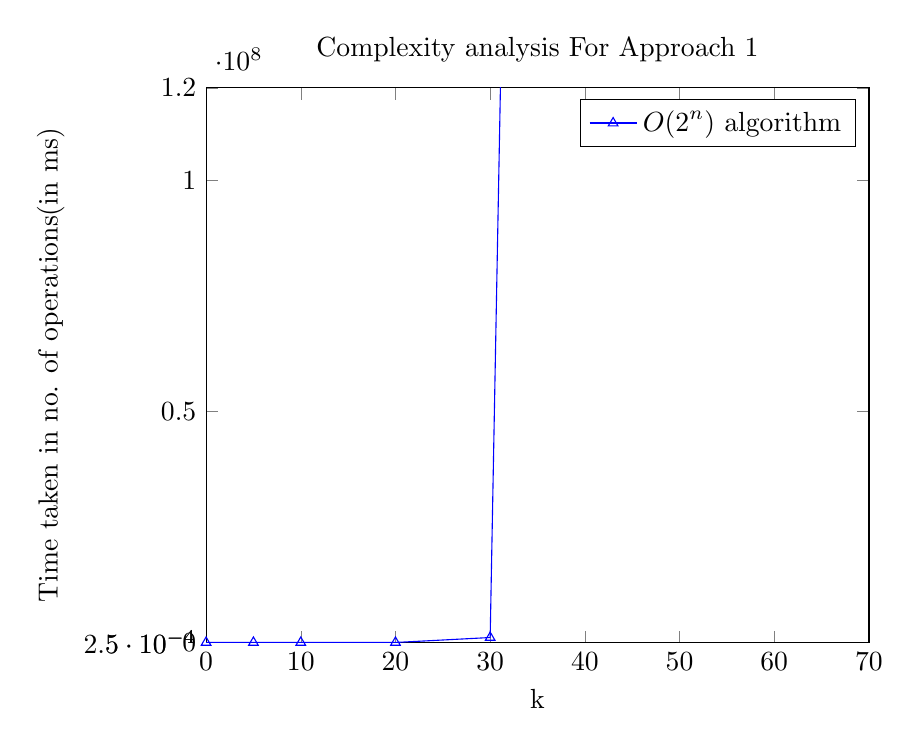
\begin{tikzpicture}[]
\begin{axis}[
    title={Complexity analysis For Approach 1 },
    xlabel={k},
    ylabel={Time taken in no. of operations(in ms)},
    xmin=0, xmax=70,
    ymin=0, ymax=120000000,
    xtick={0,10,20,30,40,50,60,70},
    ytick={0,25000,50000,50000000,100000000,120000000}
]

\addplot[
    color=blue,
    mark=triangle,
    ]
    coordinates {
    (0,0)(5,0.032)(10,1.024)(20,1048.576)(30,1073741.576)(40,1099511627.776)
    };
    \legend{$\displaystyle{O}{\left({2}^{n}\right)}$ algorithm}
   \end{axis}
   
\end{tikzpicture}



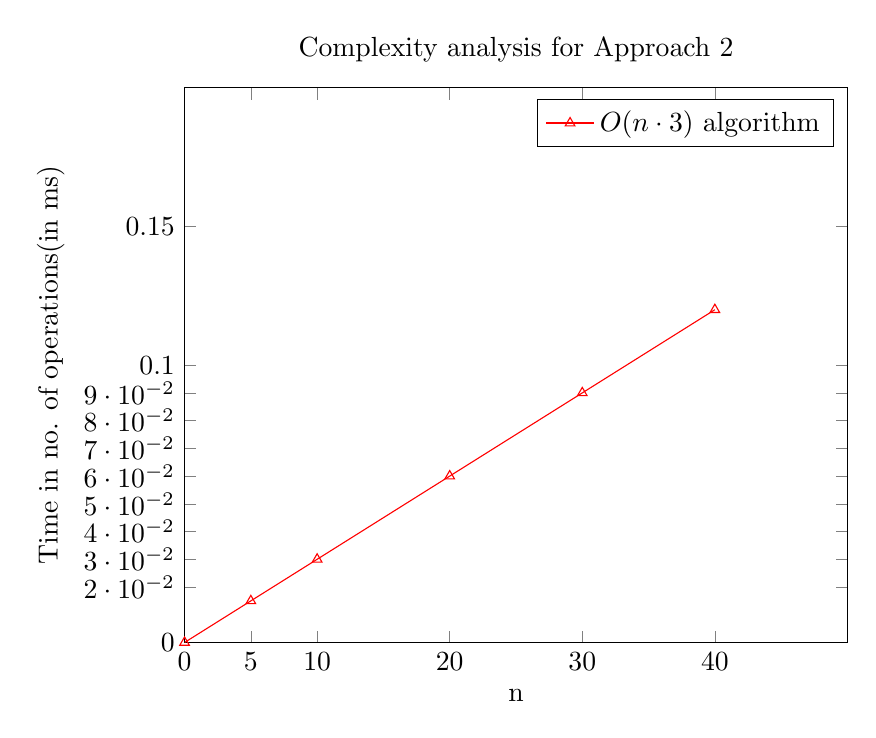
\begin{tikzpicture}
\begin{axis}[
    title={Complexity analysis for Approach 2},
    xlabel={n},
    ylabel={Time in no. of operations(in ms)},
    xmin=0, xmax=50,
    ymin=0, ymax=0.2,
    xtick={0,5,10,20,30,40},
    ytick={0,0.02,0.03,0.04,0.05,0.06,0.07,0.08,0.09,0.1,0.15},
]

\addplot[
    color=red,
    mark=triangle,
    ]
    coordinates {
    (0,0)(5,0.015)(10,0.03)(20,0.06)(30,0.090)(40,0.12)
    };
    \legend{$\displaystyle{O}{\left({n}\cdot{3}\right)}$ algorithm}
  \end{axis}
  \end{tikzpicture}
  
\section{Conclusion}
Above two methods have different time complexities and meet to fulfill the problem statement. The order in which they are good can be listed as:
\\I. Approach 2
\\II. Approach 1
\\Based on the time complexities.
\section{REFERENCES}
\begin{enumerate}
\item Utkarsh Trivedi, ’Longest Zig-Zag Subsequence’, GeeksforGeeks, 2018. [Online]. [Accessed: 27-Mar-2021]
\end{enumerate}

\end{document}
